\documentclass[]{article}
\usepackage{lmodern}
\usepackage{amssymb,amsmath}
\usepackage{ifxetex,ifluatex}
\usepackage{fixltx2e} % provides \textsubscript
\ifnum 0\ifxetex 1\fi\ifluatex 1\fi=0 % if pdftex
  \usepackage[T1]{fontenc}
  \usepackage[utf8]{inputenc}
\else % if luatex or xelatex
  \ifxetex
    \usepackage{mathspec}
  \else
    \usepackage{fontspec}
  \fi
  \defaultfontfeatures{Ligatures=TeX,Scale=MatchLowercase}
\fi
% use upquote if available, for straight quotes in verbatim environments
\IfFileExists{upquote.sty}{\usepackage{upquote}}{}
% use microtype if available
\IfFileExists{microtype.sty}{%
\usepackage{microtype}
\UseMicrotypeSet[protrusion]{basicmath} % disable protrusion for tt fonts
}{}
\usepackage[margin=1in]{geometry}
\usepackage{hyperref}
\hypersetup{unicode=true,
            pdftitle={Lab 3: Reducing Crime},
            pdfauthor={Madeleine Bulkow, Kim Darnell, Alla Hale, Emily Rapport},
            pdfborder={0 0 0},
            breaklinks=true}
\urlstyle{same}  % don't use monospace font for urls
\usepackage{color}
\usepackage{fancyvrb}
\newcommand{\VerbBar}{|}
\newcommand{\VERB}{\Verb[commandchars=\\\{\}]}
\DefineVerbatimEnvironment{Highlighting}{Verbatim}{commandchars=\\\{\}}
% Add ',fontsize=\small' for more characters per line
\usepackage{framed}
\definecolor{shadecolor}{RGB}{248,248,248}
\newenvironment{Shaded}{\begin{snugshade}}{\end{snugshade}}
\newcommand{\KeywordTok}[1]{\textcolor[rgb]{0.13,0.29,0.53}{\textbf{#1}}}
\newcommand{\DataTypeTok}[1]{\textcolor[rgb]{0.13,0.29,0.53}{#1}}
\newcommand{\DecValTok}[1]{\textcolor[rgb]{0.00,0.00,0.81}{#1}}
\newcommand{\BaseNTok}[1]{\textcolor[rgb]{0.00,0.00,0.81}{#1}}
\newcommand{\FloatTok}[1]{\textcolor[rgb]{0.00,0.00,0.81}{#1}}
\newcommand{\ConstantTok}[1]{\textcolor[rgb]{0.00,0.00,0.00}{#1}}
\newcommand{\CharTok}[1]{\textcolor[rgb]{0.31,0.60,0.02}{#1}}
\newcommand{\SpecialCharTok}[1]{\textcolor[rgb]{0.00,0.00,0.00}{#1}}
\newcommand{\StringTok}[1]{\textcolor[rgb]{0.31,0.60,0.02}{#1}}
\newcommand{\VerbatimStringTok}[1]{\textcolor[rgb]{0.31,0.60,0.02}{#1}}
\newcommand{\SpecialStringTok}[1]{\textcolor[rgb]{0.31,0.60,0.02}{#1}}
\newcommand{\ImportTok}[1]{#1}
\newcommand{\CommentTok}[1]{\textcolor[rgb]{0.56,0.35,0.01}{\textit{#1}}}
\newcommand{\DocumentationTok}[1]{\textcolor[rgb]{0.56,0.35,0.01}{\textbf{\textit{#1}}}}
\newcommand{\AnnotationTok}[1]{\textcolor[rgb]{0.56,0.35,0.01}{\textbf{\textit{#1}}}}
\newcommand{\CommentVarTok}[1]{\textcolor[rgb]{0.56,0.35,0.01}{\textbf{\textit{#1}}}}
\newcommand{\OtherTok}[1]{\textcolor[rgb]{0.56,0.35,0.01}{#1}}
\newcommand{\FunctionTok}[1]{\textcolor[rgb]{0.00,0.00,0.00}{#1}}
\newcommand{\VariableTok}[1]{\textcolor[rgb]{0.00,0.00,0.00}{#1}}
\newcommand{\ControlFlowTok}[1]{\textcolor[rgb]{0.13,0.29,0.53}{\textbf{#1}}}
\newcommand{\OperatorTok}[1]{\textcolor[rgb]{0.81,0.36,0.00}{\textbf{#1}}}
\newcommand{\BuiltInTok}[1]{#1}
\newcommand{\ExtensionTok}[1]{#1}
\newcommand{\PreprocessorTok}[1]{\textcolor[rgb]{0.56,0.35,0.01}{\textit{#1}}}
\newcommand{\AttributeTok}[1]{\textcolor[rgb]{0.77,0.63,0.00}{#1}}
\newcommand{\RegionMarkerTok}[1]{#1}
\newcommand{\InformationTok}[1]{\textcolor[rgb]{0.56,0.35,0.01}{\textbf{\textit{#1}}}}
\newcommand{\WarningTok}[1]{\textcolor[rgb]{0.56,0.35,0.01}{\textbf{\textit{#1}}}}
\newcommand{\AlertTok}[1]{\textcolor[rgb]{0.94,0.16,0.16}{#1}}
\newcommand{\ErrorTok}[1]{\textcolor[rgb]{0.64,0.00,0.00}{\textbf{#1}}}
\newcommand{\NormalTok}[1]{#1}
\usepackage{graphicx,grffile}
\makeatletter
\def\maxwidth{\ifdim\Gin@nat@width>\linewidth\linewidth\else\Gin@nat@width\fi}
\def\maxheight{\ifdim\Gin@nat@height>\textheight\textheight\else\Gin@nat@height\fi}
\makeatother
% Scale images if necessary, so that they will not overflow the page
% margins by default, and it is still possible to overwrite the defaults
% using explicit options in \includegraphics[width, height, ...]{}
\setkeys{Gin}{width=\maxwidth,height=\maxheight,keepaspectratio}
\IfFileExists{parskip.sty}{%
\usepackage{parskip}
}{% else
\setlength{\parindent}{0pt}
\setlength{\parskip}{6pt plus 2pt minus 1pt}
}
\setlength{\emergencystretch}{3em}  % prevent overfull lines
\providecommand{\tightlist}{%
  \setlength{\itemsep}{0pt}\setlength{\parskip}{0pt}}
\setcounter{secnumdepth}{0}
% Redefines (sub)paragraphs to behave more like sections
\ifx\paragraph\undefined\else
\let\oldparagraph\paragraph
\renewcommand{\paragraph}[1]{\oldparagraph{#1}\mbox{}}
\fi
\ifx\subparagraph\undefined\else
\let\oldsubparagraph\subparagraph
\renewcommand{\subparagraph}[1]{\oldsubparagraph{#1}\mbox{}}
\fi

%%% Use protect on footnotes to avoid problems with footnotes in titles
\let\rmarkdownfootnote\footnote%
\def\footnote{\protect\rmarkdownfootnote}

%%% Change title format to be more compact
\usepackage{titling}

% Create subtitle command for use in maketitle
\newcommand{\subtitle}[1]{
  \posttitle{
    \begin{center}\large#1\end{center}
    }
}

\setlength{\droptitle}{-2em}

  \title{Lab 3: Reducing Crime}
    \pretitle{\vspace{\droptitle}\centering\huge}
  \posttitle{\par}
  \subtitle{w203 Summer 2018}
  \author{Madeleine Bulkow, Kim Darnell, Alla Hale, Emily Rapport}
    \preauthor{\centering\large\emph}
  \postauthor{\par}
      \predate{\centering\large\emph}
  \postdate{\par}
    \date{\today}


\begin{document}
\maketitle

\subsection{1. Introduction}\label{introduction}

As advisees to political campaigns for state and local office in North
Carolina (NC), we believe that the crime rates across the state should
be of central concern to any candidate. State and local governments
desire to control the crime rate, and rigorous data analysis is needed
to understand the factors that contribute to crime in different parts of
the state. This report examines the available crime data and attempts to
answer the following research question: \emph{What variables are
associated with crime rates across counties in North Carolina?} Based on
this analysis, we generate several policy suggestions applicable to
candidates seeking or defending office in North Carolina.

\subsection{2. Variable Definitions and
Assumptions}\label{variable-definitions-and-assumptions}

The data analyzed in this report were collected as part of a multi-year
study on crime by Cornwell and Trumball, originally published in 1994.
The data include various factors potentially related to crime for 90 of
the 100 counties in North Carolina. Because of legal limitations on
access to the full dataset, this report will focus exculsively on the
opensource data from 1987. As such, our findings and recommendations
apply only to the North Carolina of the late 1980s.

The dataset includes the following variables, which we present with
definitions and assumptions:

\textbf{county}: An integer code indicating which North Carolina county
a given row in the datafile represents. Review of relevant factors
suggests that these integers are FIPS codes, which are standard county
identification codes generated by the Environmental Protection Agency
(see \url{http://enacademic.com/dic.nsf/enwiki/49697} for details on
FIPS codes for the state, including detailed maps).

\textbf{year}: A value of 1987 for all data points.

\textbf{crmrte}: The ratio of crimes committed per person, taken from
the FBI's Uniform Crime Reports.

\textbf{prbarr}: The ratio of arrests to offenses, taken from the FBI's
Uniform Crime Reports.

\textbf{prbconv}: The ratio of convictions to arrests. Arrest data is
taken from the FBI's Uniform Crime Reports. Conviction data is taken
from the North Carolina Department of Correction.

\textbf{prbpris}: The ratio of prison sentences to convictions, taken
from the North Carolina Department of Correction.

\textbf{avgsen}: The average prison sentence in days; we assume these
data come from the North Carolina Department of Correction.

\textbf{polpc}: The number of police officers per capita, computed using
the FBI's police agency employee counts.

\textbf{density}: The number of 100 people per square mile.

\textbf{taxpc}: The tax revenue per capita; we assume that this refers
to taxes assessed in units of \$100 dollars at the state level or lower.

\textbf{west}: An indicator code specifying whether county is in Western
North Carolina (1 if yes, 0 if no).

\textbf{central}: An indicator code specifying whether county is in
Central North Carolina (1 if yes, 0 if no).

\textbf{urban}: An indicator code specifying whether county is urban,
defined by whether the county is in a Standard Metropolitan Statistical
Area as defined by the U.S. Census (see
\url{https://www.encyclopedia.com/finance/finance-and-accounting-magazines/standard-metropolitan-statistical-areas}).

\textbf{pctmin80}: The percentage of population that belongs to a
non-White racial group according to the 1980 U.S. Census.

\textbf{mix}: The ratio of face-to-face offenses (e.g., physical
assault) to other offenses (e.g., automobile theft).

\textbf{pctymle}: The percentage of young males, defined as proportion
of population that is male between the ages of 15 and 24, according to
the 1980 U.S. Census data.

The remaining variables represent weekly wages in particular industries,
as provided by the North Carolina Employment Security Commission:

\textbf{wcon}: construction

\textbf{wtuc}: transit, utilities, and communication

\textbf{wtrd}: wholesale, retail trade

\textbf{wfir}: finance, insurance, real estate

\textbf{wser}: service industry

\textbf{wmfg}: manufacturing

\textbf{wfed}: federal employees

\textbf{wsta}: state employees

\textbf{wloc}: local government employees

We start by evaluating the available data, cleaning it by removing
anomolous values, and transforming relevant variables.

\begin{Shaded}
\begin{Highlighting}[]
\CommentTok{# Import the data}
\NormalTok{df =}\StringTok{ }\KeywordTok{read.csv}\NormalTok{(}\StringTok{"crime_v2.csv"}\NormalTok{)}
\end{Highlighting}
\end{Shaded}

\subsection{Data Adjustments and
Anomalies}\label{data-adjustments-and-anomalies}

The dataset has several ratio variables, including \textbf{prbarr},
\textbf{prbpris}, \textbf{pctymle}, and \textbf{mix}, that recorded as
decimal values between 0-1. To facilitate comparing the coefficients for
these variables more easily with other numerical values in the dataset,
we converted their scale to 0-100, as in percentages. The exception to
this approach was \emph{prbconv}, which reflects the ratio of
convictions to arrests. This variable has several values that are
greater than 1, indicating that there are counties where individuals are
convicted of more crimes than they were intially arrested for. Modifying
the scale of this variable did not seem to improve its interpretablity,
so it was unchanged.

The variable \emph{polpc} represents the number of police officers per
known resident in a county, which is somewhat intangible on an
individual scale. That is, it is awkward to refer to ``.004 police
officers per person.'' To address this, we multiplied the scores for
this variable by 1000, permitting descriptions such as ``4 police
officers per 1000 people.''

There is one county, Madison County (FIPS 115), for which the
\emph{prbarr} value is greater than 100\%. This anomaly could reflect an
error in data gathering or recording, but it may also reflect that it is
common for individuals in this county to be arrested with greater
frequency than they commit specific offenses. We did not remove,
replace, or adjust this score.

The data for Wilkes Country (FIPS 193) are given twice. We removed one
set of these values so that they would not unduly affect the overall
analysis. In addition, there were six rows in the dataset that had no
values for any variable. We assumed these rows were unintentionally
included and removed all of them.

Data were not provided for the following counties (FIPS county codes are
provide in parentheses): Camden (29), Carteret (31), Clay (43), Gates
(73), Graham (75), Hyde (95), Jones (103), Mitchell (121), Tyrrell
(177), and Yancey (199). We do not know why these cases were omitted
from the original dataset, nor can we say for certain the extent to
which the omission of 1/10 counties across the state might affect the
effectiveness of our recommendations. However, a review of 2012
population estimates for the omitted counties (see
\url{http://us-places.com/North-Carolina/population-by-County.htm})
indicate that 9/10 are ranked between 86-100 of the 100 counties in
overall population. The remaining omitted county is ranked 37th overall
in population in the state and is close to several major metropolitan
areas in the Northeast. This pattern of omission draws our attention to
the variable of \emph{density}, which we will consider with particular
care.

\begin{Shaded}
\begin{Highlighting}[]
\CommentTok{# Clean the data}

\NormalTok{## Reassign the dataframe to a working variable}
\NormalTok{df_calc <-}\StringTok{ }\NormalTok{df}

\CommentTok{# Convert the prbarr, prbpris, and pctymle variables from decimals to percentages}
\NormalTok{df_calc}\OperatorTok{$}\NormalTok{prbarr <-}\StringTok{ }\NormalTok{df}\OperatorTok{$}\NormalTok{prbarr }\OperatorTok{*}\StringTok{ }\DecValTok{100}
\NormalTok{df_calc}\OperatorTok{$}\NormalTok{prbpris <-}\StringTok{ }\NormalTok{df}\OperatorTok{$}\NormalTok{prbpris }\OperatorTok{*}\StringTok{ }\DecValTok{100}
\NormalTok{df_calc}\OperatorTok{$}\NormalTok{pctymle <-}\StringTok{ }\NormalTok{df}\OperatorTok{$}\NormalTok{pctymle }\OperatorTok{*}\StringTok{ }\DecValTok{100}

\CommentTok{# Convert the mix variable from decimals to percentage}
\NormalTok{df_calc}\OperatorTok{$}\NormalTok{mix <-}\StringTok{ }\NormalTok{df}\OperatorTok{$}\NormalTok{mix }\OperatorTok{*}\StringTok{ }\DecValTok{100}

\CommentTok{# Convert the polpc variable from decimals to number of police per 1000 people}
\NormalTok{df_calc}\OperatorTok{$}\NormalTok{polpc <-}\StringTok{ }\NormalTok{df}\OperatorTok{$}\NormalTok{polpc }\OperatorTok{*}\StringTok{ }\DecValTok{1000}

\CommentTok{# Convert the prbconv variable from integer to numeric}
\NormalTok{df_calc}\OperatorTok{$}\NormalTok{prbconv <-}\StringTok{ }\KeywordTok{as.numeric}\NormalTok{(}\KeywordTok{levels}\NormalTok{(df}\OperatorTok{$}\NormalTok{prbconv)[df}\OperatorTok{$}\NormalTok{prbconv])}
\end{Highlighting}
\end{Shaded}

\begin{verbatim}
## Warning: NAs introduced by coercion
\end{verbatim}

\begin{Shaded}
\begin{Highlighting}[]
\CommentTok{#remove row 89, which is a duplicate of row 88 (Madison County, FIPS 193)}
\NormalTok{df_clean <-}\StringTok{ }\NormalTok{df_calc[}\OperatorTok{-}\KeywordTok{c}\NormalTok{(}\DecValTok{89}\NormalTok{), ]}

\CommentTok{#remove rows with no data (i.e., all NA values)}
\NormalTok{df_clean <-}\StringTok{ }\NormalTok{df_clean[}\OperatorTok{-}\KeywordTok{c}\NormalTok{(}\DecValTok{91}\OperatorTok{:}\DecValTok{97}\NormalTok{), ]}
\end{Highlighting}
\end{Shaded}

\subsection{3. Understanding Crime Rate}\label{understanding-crime-rate}

Our central goal for this analysis is to determine what variables are
most clearly predictive of crime across the different counties of North
Carolina. For this reason, we will use \textbf{crmrte} as our primary
outcome variable.

To begin, we examine the distribution of \textbf{crmrte} to determine
its center and variability, based on data from 90 counties; there were
no missing cases. This reveals that value of \textbf{crmrte} ranges from
approximately 0.006 to .099, with a mean of approximately .034. In
practical terms, this means that the crime rate in North Carolina for
1987 varies from approximately 6-99 crimes per 1000 people, with an
average of 3.4 crimes per 1000 people.

\begin{Shaded}
\begin{Highlighting}[]
\KeywordTok{summary}\NormalTok{(df_clean}\OperatorTok{$}\NormalTok{crmrte)}
\end{Highlighting}
\end{Shaded}

\begin{verbatim}
##     Min.  1st Qu.   Median     Mean  3rd Qu.     Max. 
## 0.005533 0.020604 0.030002 0.033510 0.040249 0.098966
\end{verbatim}

\begin{Shaded}
\begin{Highlighting}[]
\KeywordTok{length}\NormalTok{(df_clean}\OperatorTok{$}\NormalTok{crmrte)}
\end{Highlighting}
\end{Shaded}

\begin{verbatim}
## [1] 90
\end{verbatim}

A histogram of the data reveals that the crime rate data are positively
skewed, with the majority of counties having a crime rate between 1-4\%
(i.e., 1-4 crimes per 100 people). The extended right tail indicates
that a few counties have substantially higher crime rates, with some
between 8-10\% (i.e., 8-10 crimes per 100 people).

\begin{Shaded}
\begin{Highlighting}[]
\KeywordTok{hist}\NormalTok{(df_clean}\OperatorTok{$}\NormalTok{crmrte, }
     \DataTypeTok{main=}\StringTok{"County Crime Rates in 1987 North Carolina"}\NormalTok{, }
     \DataTypeTok{xlab=} \StringTok{"Crimes Committed per Person"}\NormalTok{, }
     \DataTypeTok{ylab=} \StringTok{"Number of Counties"}\NormalTok{)}
\end{Highlighting}
\end{Shaded}

\includegraphics{Lab03_Bulkow_Darnell_Hale_Rapport_files/figure-latex/unnamed-chunk-4-1.pdf}

Although constituents are concerned with the crime rate in general, our
experience suggests that they are often more concerned about crimes that
result in personal physical harm to people (i.e., ``personal crime'',
with a focus on ``violent crime'') than those that simply result in loss
or damage to property (i.e., ``property crime''). For this reason, the
effective political candidate must not simply focus on policies for
reducing the general crime rate, but must consider how to perceptably
reduce the personal crime rate, and especially the violent crime rate,
for their constituents.

In the current dataset, we may generally access the distinction between
personal and property crime by examining the different rates of
``face-to-face crime''``, which reflects crime directly involving
victims, and''other" crime, which includes crime not directly involving
victims. This permits us to address a corollary to our primary research
question, namely: \emph{What are the variables associated with the
}face-to-face* crime rates across counties in North Carolina?*

Extracting the face-to-face crime rate involves manipulations on
\textbf{crmrte} involving \textbf{mix}, which the reader will recall is
the ratio of face-to-face crimes to other crimes. Specifically, we begin
by assuming that the total crime rate equals the face-to-face crime rate
\(+\) the other crime rate. A somewhat tortuous manipulation, detailed
below, allows us to calculate the ratio of face-to-face crimes among all
crimes committed for each country in the dataset.

\begin{align}
\frac{\text{face-to-face}}{\text{total}} &= 1 - \frac{\text{other}}{\text{total}} \\
&= 1 - \frac{\text{other}}{\text{face-to-face}+\text{other}} \\
&= 1 - \frac{1}{\frac{\text{face-to-face}+\text{other}}{\text{other}}}\\
&= 1 - \frac{1}{\frac{\text{face-to-face}}{\text{other}}+1}\\
&= 1 - \frac{1}{\text{mix}+1}
\end{align}

We use the resulting fraction, multiplied with the value for
\textbf{crmrte} for a given county, to generate the face-to-face crime
rate (i.e., \textbf{f2fcrmrte}) for that county.

\begin{Shaded}
\begin{Highlighting}[]
\CommentTok{# Calculate the face-to-face crime rate}
\NormalTok{df_clean}\OperatorTok{$}\NormalTok{ftfcrmrte <-}\StringTok{ }\NormalTok{df_clean}\OperatorTok{$}\NormalTok{crmrte }\OperatorTok{*}\StringTok{ }\NormalTok{(}\DecValTok{1}\OperatorTok{-}\DecValTok{1}\OperatorTok{/}\NormalTok{(df_clean}\OperatorTok{$}\NormalTok{mix}\OperatorTok{+}\DecValTok{1}\NormalTok{))}
\CommentTok{# Examine the distribution}
\KeywordTok{summary}\NormalTok{(df_clean}\OperatorTok{$}\NormalTok{ftfcrmrte)}
\end{Highlighting}
\end{Shaded}

\begin{verbatim}
##    Min. 1st Qu.  Median    Mean 3rd Qu.    Max. 
## 0.00503 0.01886 0.02692 0.03048 0.03649 0.09343
\end{verbatim}

\begin{Shaded}
\begin{Highlighting}[]
\KeywordTok{hist}\NormalTok{(df_clean}\OperatorTok{$}\NormalTok{ftfcrmrte, }
     \DataTypeTok{main=}\StringTok{"Face-to-Face Crime Rates"}\NormalTok{, }
     \DataTypeTok{xlab=} \StringTok{"Crimes Committed per Person"}\NormalTok{, }
     \DataTypeTok{ylab=} \StringTok{"Number of Counties"}\NormalTok{)}
\end{Highlighting}
\end{Shaded}

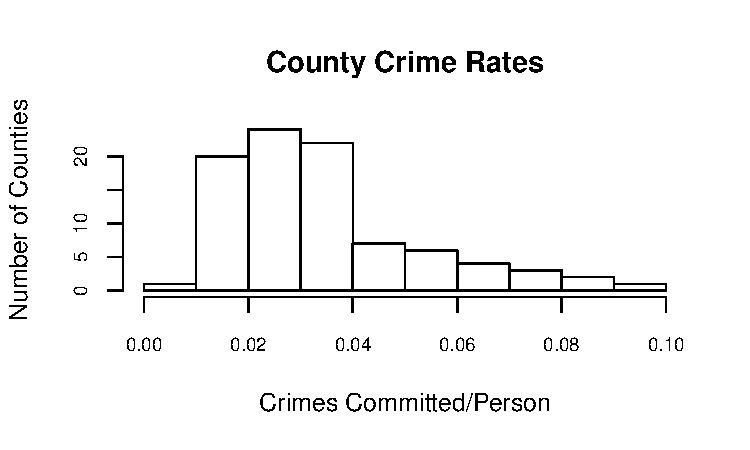
\includegraphics{Lab03_Bulkow_Darnell_Hale_Rapport_files/figure-latex/unnamed-chunk-5-1.pdf}

\begin{Shaded}
\begin{Highlighting}[]
\NormalTok{df_clean}\OperatorTok{$}\NormalTok{crmrte_ratio <-}\StringTok{ }\DecValTok{1}\OperatorTok{-}\DecValTok{1}\OperatorTok{/}\NormalTok{(df_clean}\OperatorTok{$}\NormalTok{mix}\OperatorTok{+}\DecValTok{1}\NormalTok{)}
\KeywordTok{hist}\NormalTok{(df_clean}\OperatorTok{$}\NormalTok{crmrte_ratio,}
     \DataTypeTok{main=} \StringTok{"County Crime Rates in 1987 North Carolina"}\NormalTok{,}
     \DataTypeTok{xlab=} \StringTok{"Face-to-Face Crimes/Total Crimes"}\NormalTok{,}
     \DataTypeTok{ylab=} \StringTok{"Number of Counties"}\NormalTok{)}
\end{Highlighting}
\end{Shaded}

\includegraphics{Lab03_Bulkow_Darnell_Hale_Rapport_files/figure-latex/unnamed-chunk-5-2.pdf}

We note that the distribution of the face-to-face crime rate is similar,
but not identical to, the general crime rate. In particular,
\textbf{f2rcrmrte} has a slightly lower mean of 3\% (i.e., an average of
3 personal crimes per 100 people), and a range of 0.5\% to 9.3\% (i.e.,
5-93 crimes per 1000 people). The similarity of the two variables
suggests that it is appropriate for our analysis to focus primarily on
the more general \textbf{crmrte}, then extended secondarily to
\textbf{f2fcrmrte} in the context of policy recommendations.

\subsection{4. Models and Assumptions}\label{models-and-assumptions}

For analyses of this type, we use ordinarly least squares (OLS)
regression, also known as multiple linear regression, to determine what
associations, if any, exist among the variables in the dataset. We
identify a variable to be explained -- the ``outcome'' variable -- and
then perform analyses involving different combinations of
``explanatory'' (or ``predictor'') variables from the dataset to see the
degree to which those variables and combinations can predict the
observed outcomes. Each set of calculations, involving the outcome
variable and a specific combination of explanatory variables, is
referred to as a ``model''. Models typically build on each other,
starting with a few explanatory variables that are determined to be
particularly important, and are subsequently extended by adding more
explanatory variables in order to increase the predictive value relative
to the outcome variable.

In addition to the outcome and explanatory variables, each model
contains some degree of statistical error, typically represented as
\emph{u}. This error represents an unknown value of the difference
between the true value of the variables in the world and the values for
those variables given in the dataset. For example, there is some
difference between the actual crime rate across counties in North
Carolina and the measures we have for that crime rate in the current
dataset, because the dataset does not reflect every single crime that
was committed in every single county across the entire state during the
time period of interest. To the extent that the variables in the dataset
were well designed and implemented, and the values for those variables
accurately and thoroughly gathered, the statistical error will be
smaller. All statistical models involve some degree of statistical
error.

Other statistical terms that may be useful for the reader to be familiar
with include:

\begin{itemize}
  \item "coefficient": A value multiplied by a variable (e.g., in 5x, 5 is a coeffient)
  \item "fitted value": A predicted value for a variable that is generated when trying to find the best fit for the value into a particular regression equation. 
  \item "residual": The difference between the observed value of a variable and the predicted value for that same variable; typically represented as *e*. Each data point has one residual.
\end{itemize}

For the current analysis, we model the factors contributing to crime
rate across the counties of North Carolina in five stages, resulting in
five models. Each of these models is described below.

\begin{itemize}
  \item \underline{Model 1} includes only the variables we believe to be the main predictors of crime rate (**crmrte**): population density (**density**), tax per capita (**taxpc**), and percentage of young males in the population (**pctymle**).  
  \item \underline{Model 2} includes the factors from Model 1 as well as several others that we believe contribute meaningfully to crime rate, including location in the state (**west**), the number of police per 1000 residents (**polpc**), the ratio of arrests to offenses (**prbarr**), the ratio of convictions to arrests (**prbconv**), and the proportion of non-White minorities (**pctmin80**).  
  \item \underline{Model 3} builds on Model 2 by adding more information about the location of the county (**central**), the ratio of prison sentences to convictions (**prbpris**), and the average length of prison sentence (**avgsen**).  
  \item \underline{Model 4} builds on Model 3 and adds all other explanatory variables in the dataset that are not covariant with any explanatory variables already included. 
  \item\underline{Model 5} explores whether predictors we identify for general crime rate are comparably effective for explaining the rate of face-to-face crime across counties in North Carolina by using the secondary outcome variable **f2fcrmrte**, based on **crmrate** and **mix**.
\end{itemize}

Each of our models will be assessed to determine it's consistency with
the following assumptions, which are standard for classic linear
regression models like these. The statistical quality of our findings is
dependent on these assumptions being met.

\begin{itemize}
  \item \underline{Assumption 1}: Linearity in parameters, such that each fit model has slope coefficients that are linear multipliers of the associated predictor variables. 
  \item \underline{Assumption 2}: Random sampling, such that the data points are independent and identically distributed. 
  \item \underline{Assumption 3}: No perfect collinearity, such that none of the variables in the sample is a constant and there is no exact linear relationship among the predictor variables.
  \item \underline{Assumption 4}: Zero conditional mean, such that the statistical error in the model has an expected value of 0 given any values of the predictor variables.
  \item \underline{Assumption 5}: Homoskedasticity, such that the statistical error in the model has the same variance given any value of the predictor variables.
  \item \underline{Assumption 6}: Normality, such that the statistical error in the population is independent of the predictor variables and is normally distributed with zero mean and variance sigma-squared.
\end{itemize}

For each of our models, we expect a classical linear model meeting
Assumption 1; this is supported by the nature of our variables and the
type of analysis we employ.

We also expect all of our models to meet Assumption 2, regarding random
sampling, given that our dataset reflects 90 of North Carolina's 100
counties, which is very close to the overall population. As a caveat, we
note that 9/10 of the omitted counties are those for which 2012
population estimates are in the low 15\% for the state. Although it is
possible that these counties could have been omitted via an
appropriately executed random sampling procedure, the pattern inherent
in these omissions may require additional explanation or analysis,
particularly if population density emerges as a useful predictor. It is
relevant to note that in Northeast cities in the early 1980s, the rate
of violent crime, but not property crime, was correlated with population
density (see
\url{https://www.ncjrs.gov/App/Publications/abstract.aspx?ID=99314}).

Assumptions 3-6, which are dependent on the explanatory variables
involved, will be tested independently for each model. Related to this,
we note that, in some cases, it may be necessary to mathematically
transform some portion of the data (e.g., convert the values for an
explanatory variable to their logarithmic form) in order to facilitate
an assumption being met. For example, transformations are commonly used
to linearize the relationship between variables, improve
homoskedasticity, or make the data more consistent with expected
practice in a given scientific discipline. Beyond cases that have
specific statistical or theoretical motivations, we will use the data in
its original form.

\subsubsection{4.1 Model 1}\label{model-1}

An exploratory examination of the data suggest that population density,
local and state tax per capita, and the percentage of young males in the
county are strong predictors of the general crime rate. We begin by
evaluating and describing each of these predictor variables in turn.

Population density (\textbf{density}):

\begin{Shaded}
\begin{Highlighting}[]
\KeywordTok{summary}\NormalTok{(df_clean}\OperatorTok{$}\NormalTok{density)}
\end{Highlighting}
\end{Shaded}

\begin{verbatim}
##    Min. 1st Qu.  Median    Mean 3rd Qu.    Max. 
## 0.00002 0.54718 0.97925 1.43567 1.56926 8.82765
\end{verbatim}

\begin{Shaded}
\begin{Highlighting}[]
\KeywordTok{hist}\NormalTok{(df_clean}\OperatorTok{$}\NormalTok{density,}
     \DataTypeTok{main=}\StringTok{"Population Density across NC Counties"}\NormalTok{, }
     \DataTypeTok{xlab=} \StringTok{"Population Density (1/100)"}\NormalTok{, }
     \DataTypeTok{ylab=} \StringTok{"Number of Counties"}\NormalTok{,}
     \DataTypeTok{breaks =} \DecValTok{15}\NormalTok{)}
\end{Highlighting}
\end{Shaded}

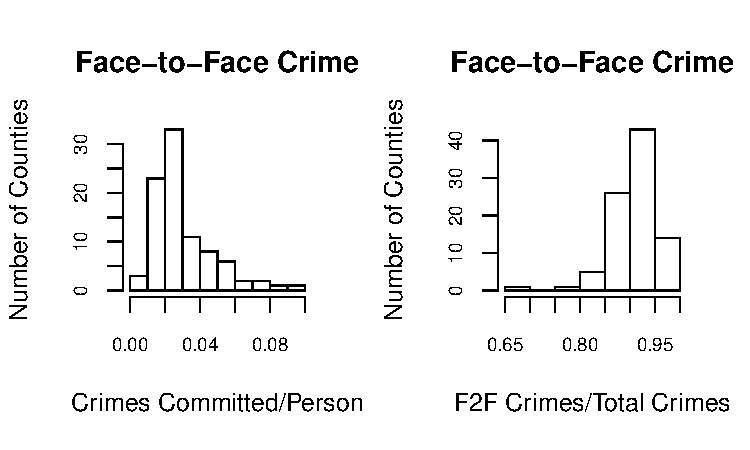
\includegraphics{Lab03_Bulkow_Darnell_Hale_Rapport_files/figure-latex/unnamed-chunk-6-1.pdf}

The value of density ranges from a score of approximately 0.002 to 880
people per square mile, with a mean of 145. The distribution of county
densities is right skewed, with most counties having a score of 200 or
fewer people per square mile.

Tax per Capita (\textbf{taxpc}):

\begin{Shaded}
\begin{Highlighting}[]
\KeywordTok{summary}\NormalTok{(df_clean}\OperatorTok{$}\NormalTok{taxpc)}
\end{Highlighting}
\end{Shaded}

\begin{verbatim}
##    Min. 1st Qu.  Median    Mean 3rd Qu.    Max. 
##   25.69   30.73   34.92   38.16   41.01  119.76
\end{verbatim}

\begin{Shaded}
\begin{Highlighting}[]
\KeywordTok{hist}\NormalTok{(df_clean}\OperatorTok{$}\NormalTok{taxpc,}
     \DataTypeTok{main=}\StringTok{"Tax per Capita Across NC Counties"}\NormalTok{, }
     \DataTypeTok{xlab=} \StringTok{"Local and State Tax per Capita (1/100)"}\NormalTok{, }
     \DataTypeTok{ylab=} \StringTok{"Number of Counties"}\NormalTok{,}
     \DataTypeTok{breaks =} \DecValTok{30}\NormalTok{)}
\end{Highlighting}
\end{Shaded}

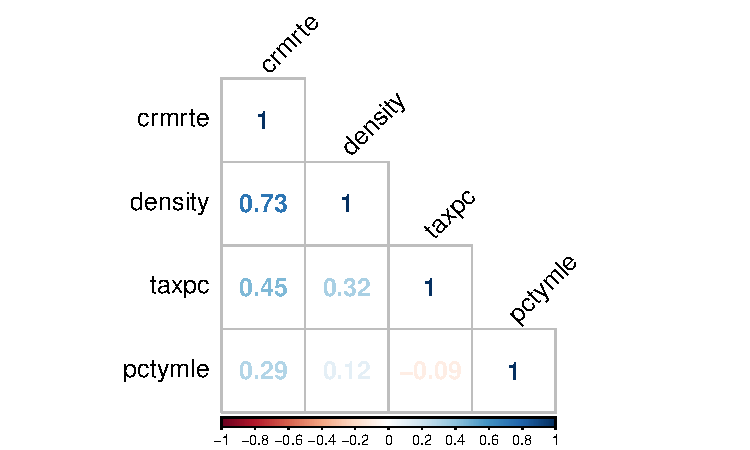
\includegraphics{Lab03_Bulkow_Darnell_Hale_Rapport_files/figure-latex/unnamed-chunk-7-1.pdf}

The cumulative value of taxes assessed at the local and state levels per
capita ranges from \$2,569 to \$11,976 per year. Once again, we see a
distribution that is right skewed, with revenue in most counties below
the mean of \$3,813 per year. The maximum value, the value for Dare
county (FIPS 55) is nearly 50\% higher than the next closest value,
suggesting that this county has an anomalously high tax rate for the
state. In fact, a review of the official website for Dare county
(\url{https://www.darenc.com/}) reveals that it has an extremely active
toursim industry and features a number of popular attractions, including
the Outer Banks beach resort area, the Wright Brothers National
Monument, the North Carolina Aquarium, and a number of other historic
and recreational sites. The high rate of tax per capita for this country
can easily be explained by taxes on activities related to toursim, such
as those appended to hotel, rental car, and park entrance fee costs.

Percentage of Young Males (\textbf{pctymle}):

\begin{Shaded}
\begin{Highlighting}[]
\KeywordTok{summary}\NormalTok{(df_clean}\OperatorTok{$}\NormalTok{pctymle)}
\end{Highlighting}
\end{Shaded}

\begin{verbatim}
##    Min. 1st Qu.  Median    Mean 3rd Qu.    Max. 
##   6.216   7.437   7.770   8.403   8.352  24.871
\end{verbatim}

\begin{Shaded}
\begin{Highlighting}[]
\KeywordTok{hist}\NormalTok{(df_clean}\OperatorTok{$}\NormalTok{pctymle,}
     \DataTypeTok{main=} \StringTok{" Percent Males Ages 15-24 across Counties"}\NormalTok{, }
     \DataTypeTok{xlab=} \StringTok{"Percent Males Ages 15-24"}\NormalTok{, }
     \DataTypeTok{ylab=} \StringTok{"Number of Counties"}\NormalTok{,}
     \DataTypeTok{breaks =} \DecValTok{30}\NormalTok{)}
\end{Highlighting}
\end{Shaded}

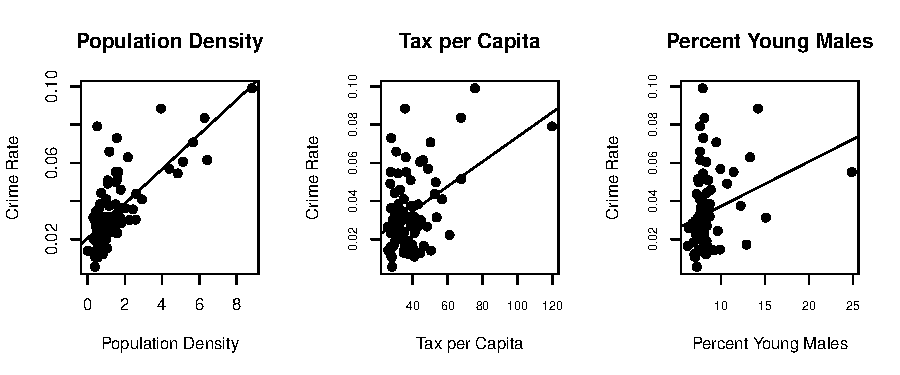
\includegraphics{Lab03_Bulkow_Darnell_Hale_Rapport_files/figure-latex/unnamed-chunk-8-1.pdf}

Across the counties of North Carolina, the percentage of males between
15-24 years of age ranges from 6.2 to 24.9. Once again, we see a
distribution that is right skewed, with the majority of counties having
fewer than the mean of 8.4\% young males. There is one extreme value:
that for Onslow county (FIPS 133). This reflects that Onslow county
includes the city of Jacksonville, which contains the United States
Marine Corps' Camp Lejeune and the New River Air Station, both of which
are inhabited predominately by males under 25 years of age.

Before we build our model, we review the matrix of scatterplots of crime
rate and the three predictor variables to assess the variables'
consistency with Assumption 3 regarding no perfect collinearity.

\begin{Shaded}
\begin{Highlighting}[]
\NormalTok{vars <-}\StringTok{ }\KeywordTok{c}\NormalTok{(}\StringTok{"crmrte"}\NormalTok{, }\StringTok{"density"}\NormalTok{, }\StringTok{"taxpc"}\NormalTok{,}\StringTok{"pctymle"}\NormalTok{)}
\KeywordTok{suppressWarnings}\NormalTok{(}\KeywordTok{scatterplotMatrix}\NormalTok{(df_clean[,vars], }\DataTypeTok{diagonal =} \KeywordTok{list}\NormalTok{(}\DataTypeTok{method=} \StringTok{"histogram"}\NormalTok{)))}
\end{Highlighting}
\end{Shaded}

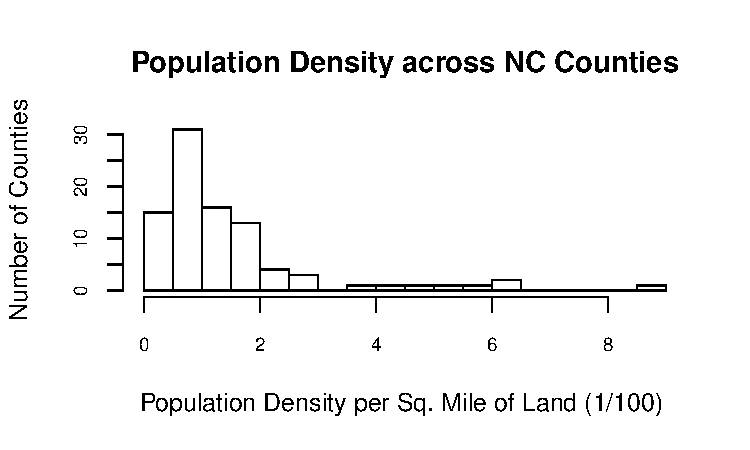
\includegraphics{Lab03_Bulkow_Darnell_Hale_Rapport_files/figure-latex/unnamed-chunk-9-1.pdf}

As previously indicated, crime rate appears predicted by each of the
three primary variables selected as evidenced by the fairly strong
positive slopes in the bivariate regressions in the scatterplot matrix.
Additionally, though \textbf{density} and \textbf{taxpc} appear to have
a positive correlation, none of the variables are collinear with any of
the others. As such, Assumption 3 is validated.

With the evaluation of the variables complete, we build Model 1, and
evaluate the Cook's Distance for the residuals:

\begin{Shaded}
\begin{Highlighting}[]
\CommentTok{# Build Model 1}
\NormalTok{model_}\DecValTok{1}\NormalTok{ =}\StringTok{ }\KeywordTok{lm}\NormalTok{(crmrte }\OperatorTok{~}\StringTok{ }\NormalTok{density }\OperatorTok{+}\StringTok{ }\NormalTok{taxpc }\OperatorTok{+}\StringTok{ }\NormalTok{pctymle, }\DataTypeTok{data =}\NormalTok{ df_clean)}
\KeywordTok{summary}\NormalTok{(model_}\DecValTok{1}\NormalTok{)}\OperatorTok{$}\NormalTok{r.square}
\end{Highlighting}
\end{Shaded}

\begin{verbatim}
## [1] 0.6404252
\end{verbatim}

\begin{Shaded}
\begin{Highlighting}[]
\KeywordTok{plot}\NormalTok{(model_}\DecValTok{1}\NormalTok{, }\DataTypeTok{which =} \DecValTok{5}\NormalTok{)}
\end{Highlighting}
\end{Shaded}

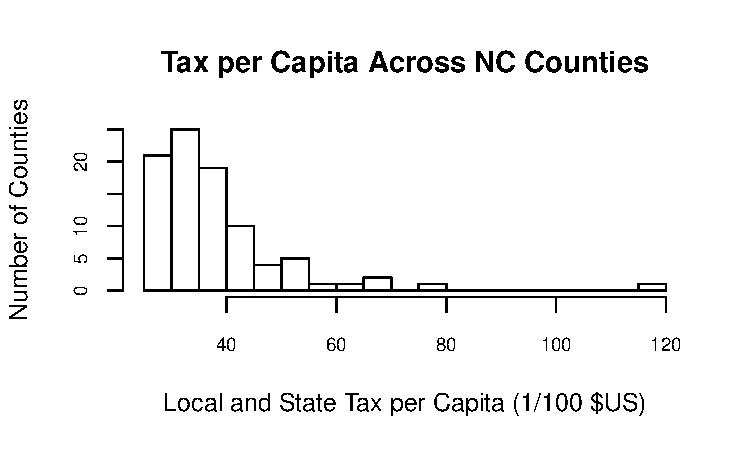
\includegraphics{Lab03_Bulkow_Darnell_Hale_Rapport_files/figure-latex/unnamed-chunk-10-1.pdf}

We find one point that has a Cook's Distance greater than 1,
corresponding to Dare county. As noted previously, Dare country has
substantially higher tax per capita than other North Carolina counties
because of tax revenue from tourism. As such, the deviation of this
single case is understandable and does not warrant its removal.

Now that the model is built, we can evaluate the validity of Assumption
4 regarding zero conditional mean. This involves demonstrating that the
expectation (i.e., mean) of the fitted values multiplied the residuals
equals 0. Given that the denominator does not matter for this particular
calculation, we can use the sum of fitted values rather than the mean.

\begin{Shaded}
\begin{Highlighting}[]
\KeywordTok{round}\NormalTok{(}\KeywordTok{sum}\NormalTok{(model_}\DecValTok{1}\OperatorTok{$}\NormalTok{residuals }\OperatorTok{*}\StringTok{ }\NormalTok{model_}\DecValTok{1}\OperatorTok{$}\NormalTok{fitted.values), }\DecValTok{15}\NormalTok{)}
\end{Highlighting}
\end{Shaded}

\begin{verbatim}
## [1] 0
\end{verbatim}

We find that the residuals times the fitted values sum to 0, indicating
that the model meets the demands of Assumption 4.

To validate the model in terms of Assumption 5 regarding
homoskedasticity, we create a plot of the residuals vs.~fitted values.
We find that the range of errors is relatively constant throughout the
range of fitted values, which supports the assumption in question.
However, we note that we have fewer data points at the higher values of
crime rate than the lower values of crime rate, so validity in this case
may be somewhat weaker than with other assumptions.

\begin{Shaded}
\begin{Highlighting}[]
\KeywordTok{plot}\NormalTok{(model_}\DecValTok{1}\NormalTok{, }\DataTypeTok{which =} \DecValTok{1}\NormalTok{)}
\end{Highlighting}
\end{Shaded}

\includegraphics{Lab03_Bulkow_Darnell_Hale_Rapport_files/figure-latex/unnamed-chunk-12-1.pdf}

To validate Assumption 6, the normality of the residuals, we looked at a
Q-Q plot of the standardized residuals, and noted the fairly straight
line for the exceptions of the tails. Normally distributed residuals
indicate that any variation that the model does not predict is likely
due to random noise. In this case, there are likely additional factors
influencing crime rate that we are not taking into account in this
model, which are biasing our coefficients. We will discuss these factors
in the section on Omitted Variables.

\begin{Shaded}
\begin{Highlighting}[]
\KeywordTok{plot}\NormalTok{(model_}\DecValTok{1}\NormalTok{, }\DataTypeTok{which=} \DecValTok{2}\NormalTok{)}
\end{Highlighting}
\end{Shaded}

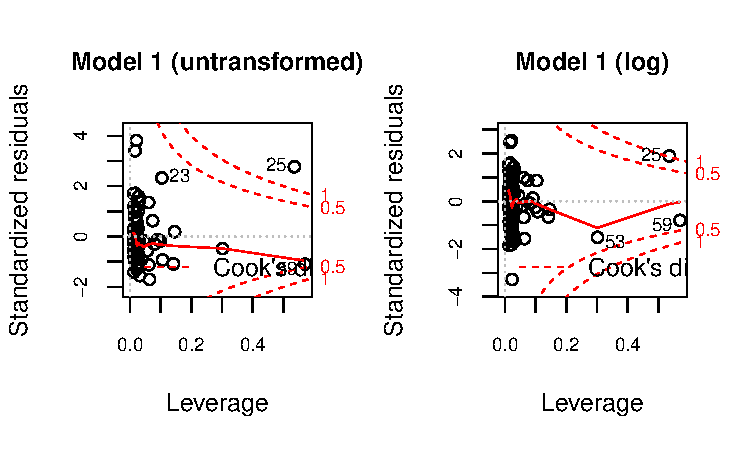
\includegraphics{Lab03_Bulkow_Darnell_Hale_Rapport_files/figure-latex/unnamed-chunk-13-1.pdf}

\subsection{Interpreting Model 1}\label{interpreting-model-1}

In Model 1, shown in Table 4.6.1, the coefficients are all positive.
This indicates that as population density, tax per capita, or the
percentage of young males increase, an associated increase occurs in
crime rate.

However, it is not the case that all of our predictor variables are
equally influencial when it comes to crime rate. Specifically, increases
in population density result in an increase of the crime rate that is an
order of magnitude greater than that for increases in tax per capita and
almost four times that generated by higher percentages of young males.
As such, this model indicates that while all of these predictors are
useful to understanding the crime rate, the candidate's energy may be
best spent on addressing crime-related concerns connected to population
density first, followed by those related to tax rate and the proportion
of young males. In the comments to follow, we highlight omitted factors
that could be influencing our findings through correlation with our
predictor variables in \textbf{bold}.

There are a number of reasons why increases in population density could
facilitate increases the crime rate. As more people live in a particular
space, there are more opportunities for them to come into conflict with
one another, to interact with others who have different access to
desireable resources an items, and to be unfamiliar with others with
whom one comes in contact day by day. As such, candidates with
constituencies in high population areas should consider addressing the
crime rate by developing policies that improve the ease with which large
numbers of people can live and move in the same space, while reducing
opportunties for conflict. \textbf{Infrastructure} projects that
increase the livability and communal nature of high population areas,
such as well-maintained public parks and recreational areas, effective
public transportation, and improved traffic and parking managment may
make it easier for residents live in close quarters with others and
reduce the number of negative experiences that might lead to criminal
behavior. Similarly, addressing problems related to
\textbf{socioeconomic inequality}, such as access to quality
\textbf{education}, employment opportunies, social support programs, and
affordable housing should also result in a reduction in crime. Last but
not least, there is the issue of anonomity. Certainly it is easier to
commit a crime against a stranger than it is a neighbor or a friend, if
only because there are fewer personal costs and a lower likelihood of
being caught. So, investing in events, facilities, and services that
encourage people to get to know and develop positive relationships with
those around them, take pride in their joint \textbf{community
membership}, and have opportunties to get to know one another as people
should also reduce crime. These might include cultural celebrations,
neighborhood vegetable gardens, or fundraising activities for an
important local cause.

The finding regarding the influence of tax per capita on crime suggests
two directions for policy to reduce crime. First, it makes sense that
areas where residents make more money would pay higher taxes \emph{and}
be more tempting targets for crime, because their higher income affords
them more access to desireable items and services. Again, this suggests
developing policies that address socioeconomic disparity so that
individuals with limited access to resources are less inspired to engage
in criminal activity to secure basic needs (e.g., money, credit cards,
items that can be fenced or pawned) from those who have more. What we do
not encourage is simply increasing the police presence in high income
areas or encouraging the police to engage in discriminatory profiling of
members of communities that are stereotypically not associated with high
socioeconomic status. These sorts of policies foment distrust among
different status communities and are likely to result in unjustified
harassment, mistreatment, and arrest of members of marginalized groups.
In fact, such policies might increase criminal activity, by discouraging
people from reporting crimes for fear of \textbf{negative police
interaction} or community backlash for ``snitching.''

The other policy direction suggested by the tax per capita result
relates to \textbf{tourism}. That is, in areas where there is a lot of
tourism, this can be seen by the community as an opportunity for good
employment and additional funding for community infrastructure and
beneficial social programs, or it can be seen as an influx of distracted
strangers with an abundance of extra money and little familiarity with
the local environment. Obviously, to the extent that tourism can be
framed as the having the former set of positive qualities for the
communities in which it occurs, the more likely crime involving tourists
is to be reduced.

With regard to the increase in crime seen with an increase in the
percentage of young males, there are a number of possibly solutions.
There is certainly immense social pressure connecting masculinity with
wealth and the ability to provide for a family, as well as factors that
socialize men to be more aggressive or violent when their needs and
wants are not immediately met. In fact, these sorts of pressures may be
even more common in communities that priortize traditional and/or
conservative social values. To the extend that a candidate's
constituency includes such communities, it could be fruitful to consider
the role that local \textbf{culture} contributes to young men committing
crimes and how providing alternative, as well as socially and personally
constructive outlets to demonstrate their masculinity could reduce
crime. Relevant policies could support educational, vocational, and
athletic programs, as well as involve young men in activies that
contribute positively to the community and encourage them to develop
rather than damage it.

\subsubsection{4.2 Model 2}\label{model-2}

Model 2 includes \textbf{west}, \textbf{polpc}, \textbf{prbarr},
\textbf{prbconv}, and \textbf{pctmin80} in addition to the three
variables from Model 1. During our initial examination of the data
(i.e., our EDA), we found that each of these had substantial
correlations with the variable of interest, crime rate.

We summarize the relationships among the new explanatory variables, with
the exception of \textbf{west} (coded effectively as ``in the western
part of the state'' or ``not in the western part of the state''). For
the dataset as a whole, 24.4 \% of all counties were coded as being
\textbf{west}.

\begin{Shaded}
\begin{Highlighting}[]
\NormalTok{vars <-}\StringTok{ }\KeywordTok{c}\NormalTok{(}\StringTok{"polpc"}\NormalTok{, }\StringTok{"prbarr"}\NormalTok{, }\StringTok{"prbconv"}\NormalTok{,}\StringTok{"pctmin80"}\NormalTok{)}
\KeywordTok{suppressWarnings}\NormalTok{(}\KeywordTok{scatterplotMatrix}\NormalTok{(df_clean[,vars], }
                                   \DataTypeTok{diagonal =} \KeywordTok{list}\NormalTok{(}\DataTypeTok{method =} \StringTok{"histogram"}\NormalTok{)))}
\end{Highlighting}
\end{Shaded}

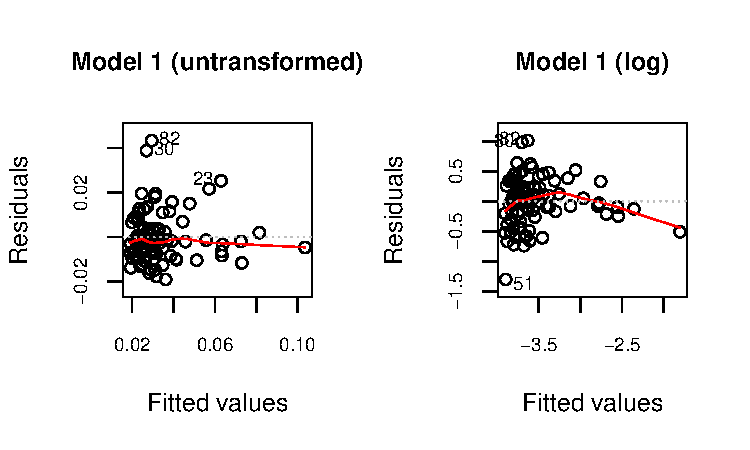
\includegraphics{Lab03_Bulkow_Darnell_Hale_Rapport_files/figure-latex/unnamed-chunk-14-1.pdf}

The matrix plot shows little to no collinearity among the considered
variables, validating Assumption 3.

\begin{Shaded}
\begin{Highlighting}[]
\CommentTok{# Build Model 2}
\NormalTok{model_}\DecValTok{2}\NormalTok{ =}\StringTok{ }\KeywordTok{lm}\NormalTok{(crmrte }\OperatorTok{~}\StringTok{ }\NormalTok{density }\OperatorTok{+}\StringTok{ }\NormalTok{taxpc }\OperatorTok{+}\StringTok{ }\NormalTok{pctymle }
              \OperatorTok{+}\StringTok{ }\NormalTok{west }\OperatorTok{+}\StringTok{ }\NormalTok{polpc }\OperatorTok{+}\StringTok{ }\NormalTok{prbarr }\OperatorTok{+}\StringTok{ }\NormalTok{prbconv }\OperatorTok{+}\StringTok{ }\NormalTok{pctmin80, }
              \DataTypeTok{data =}\NormalTok{ df_clean)}
\KeywordTok{summary}\NormalTok{(model_}\DecValTok{2}\NormalTok{)}\OperatorTok{$}\NormalTok{r.square}
\end{Highlighting}
\end{Shaded}

\begin{verbatim}
## [1] 0.8240404
\end{verbatim}

\begin{Shaded}
\begin{Highlighting}[]
\KeywordTok{plot}\NormalTok{(model_}\DecValTok{2}\NormalTok{, }\DataTypeTok{which =} \DecValTok{5}\NormalTok{)}
\end{Highlighting}
\end{Shaded}

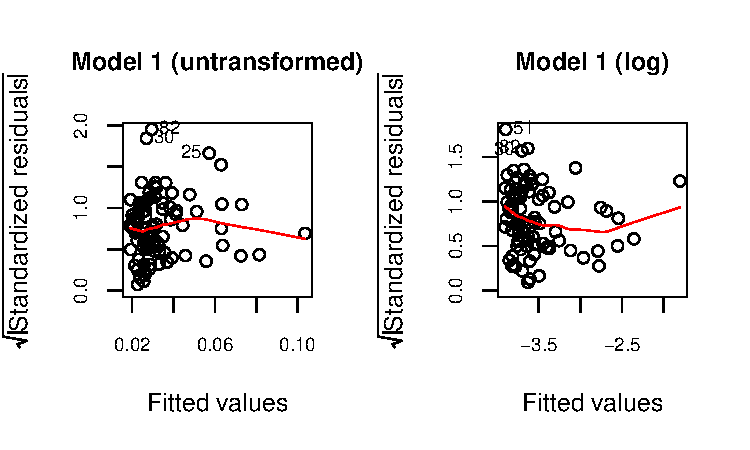
\includegraphics{Lab03_Bulkow_Darnell_Hale_Rapport_files/figure-latex/unnamed-chunk-15-1.pdf}

Unsurprisingly, the \(R^2\) increased from 0.64 to 0.82 with these
additional 5 variables included. We also note that point 25 still has
high leverage, just as in model 1. Perhaps we should study that county a
bit more closely.

We also check Assumption 4, exogeneity, by summing the product of the
residuals and fitted values and finding the sum of 0.

\begin{Shaded}
\begin{Highlighting}[]
\KeywordTok{round}\NormalTok{(}\KeywordTok{sum}\NormalTok{(model_}\DecValTok{2}\OperatorTok{$}\NormalTok{residuals }\OperatorTok{*}\StringTok{ }\NormalTok{model_}\DecValTok{2}\OperatorTok{$}\NormalTok{fitted.values), }\DecValTok{15}\NormalTok{)}
\end{Highlighting}
\end{Shaded}

\begin{verbatim}
## [1] 0
\end{verbatim}

Assumptions 5 and 6 were validated for this model as they were for Model
1. We note that the Q-Q plot of the standardized residuals appears much
closer to linear than for Model 1, indicating that we likely have most
of the significant sources of variation described by Model 2.

\begin{Shaded}
\begin{Highlighting}[]
\KeywordTok{plot}\NormalTok{(model_}\DecValTok{2}\NormalTok{, }\DataTypeTok{which=} \DecValTok{2}\NormalTok{)}
\end{Highlighting}
\end{Shaded}

\includegraphics{Lab03_Bulkow_Darnell_Hale_Rapport_files/figure-latex/unnamed-chunk-17-1.pdf}

Model 2, shown in the table in section 4.6 has positive coefficients for
\textbf{density}, \textbf{taxpc}, \textbf{pctymle}, \textbf{polpc}, and
\textbf{pctmin80} indicating that crime rate increases and these
variables increase. On the other hand, the coefficients for
\textbf{west}, \textbf{prbarr}, and \textbf{prbconv} are negative,
indicating that crime rate decreases as these increase.

The additional coefficients in this model are somewhat more challenging
to interpret than those in Model 1. It seems unlikely that the longitude
of a county would have a direct impact on its crime rate, and more
likely that there are some omitted variables associated with crime that
are more prevalent in Western counties or those with larger non-white
minority populations. Examples of these are \#\#KIM I NEED YOU HERE!\#\#

Additionally, the positive association between police per capita and
crime is noteworthy. This association should be studied further, ideally
with causal analysis, as there are plausible causal theories going in
either direction. Perhaps heightened police presence creates an
antagonistic relationship between officers and citizens, which leads to
a distrust of authority and an increase in crime; the ideal way to test
that would be to find counties with similar crime rates and other
demographics where one county changes a policing policy and the other
one does not, a natural paired experiment. However, it also seems
possible that a county that experiences more crime would choose to up
the size and acitivity of its police force in order to combat said
crime; in this case, police records and government policy could probably
help uncover this relationship. Local officials should pursue this line
of research further to make informed policy decisions about policing.

The negative correlation between crime rate and both the probability of
arrest and probability of conviction should also be studied further,
with causal analysis as described above. It could be hypothesized that
higher arrest and conviction rates deter crime. Alternatively, it could
be hypothesized that when crime rate is lower, and fewer overall crimes
are committed, it is easier to fully pursue all of the cases.

\subsubsection{4.3 Model 3}\label{model-3}

For model 3, in addition to the variables from model 2, we added the
remainder of the variables that we did not find problematic:
\textbf{central}, \textbf{avgsen}, \textbf{prison}. These variables do
not necessarily explain the crime rate well, but serve to show that
model 2 gives a reasonable explanation of the observed crime rate. We
excluded the urban variable because it is too closely related to
density, as can be seen in this scatterplot:

\begin{Shaded}
\begin{Highlighting}[]
\KeywordTok{plot}\NormalTok{(df_clean}\OperatorTok{$}\NormalTok{urban , df_clean}\OperatorTok{$}\NormalTok{density,}
     \DataTypeTok{main=} \StringTok{"Urban Density"}\NormalTok{,}
     \DataTypeTok{ylab=} \StringTok{"Density (100 people per square mile)"}\NormalTok{,}
     \DataTypeTok{xlab=} \StringTok{"Urban"}\NormalTok{)}
\KeywordTok{abline}\NormalTok{(}\KeywordTok{lm}\NormalTok{(density }\OperatorTok{~}\StringTok{ }\NormalTok{urban, }\DataTypeTok{data =}\NormalTok{ df_clean))}
\end{Highlighting}
\end{Shaded}

\includegraphics{Lab03_Bulkow_Darnell_Hale_Rapport_files/figure-latex/unnamed-chunk-18-1.pdf}

Excluded are all of the wage variables because we cannot make any
meaningful conclusions without a breakdown of what fraction of each
county are involved in each profession.

With that, we build Model 3:

\begin{Shaded}
\begin{Highlighting}[]
\CommentTok{# Build Model 3}
\NormalTok{model_}\DecValTok{3}\NormalTok{ =}\StringTok{ }\KeywordTok{lm}\NormalTok{(crmrte }\OperatorTok{~}\StringTok{ }\NormalTok{density }\OperatorTok{+}\StringTok{ }\NormalTok{taxpc }\OperatorTok{+}\StringTok{ }\NormalTok{pctymle }
             \OperatorTok{+}\StringTok{ }\NormalTok{west }\OperatorTok{+}\StringTok{ }\NormalTok{polpc }\OperatorTok{+}\StringTok{ }\NormalTok{prbarr }\OperatorTok{+}\StringTok{ }\NormalTok{prbconv }\OperatorTok{+}\StringTok{ }\NormalTok{pctmin80 }
             \OperatorTok{+}\StringTok{ }\NormalTok{central }\OperatorTok{+}\StringTok{ }\NormalTok{avgsen }\OperatorTok{+}\StringTok{ }\NormalTok{prbpris, }
             \DataTypeTok{data =}\NormalTok{ df_clean)}
\KeywordTok{summary}\NormalTok{(model_}\DecValTok{3}\NormalTok{)}\OperatorTok{$}\NormalTok{r.square}
\end{Highlighting}
\end{Shaded}

\begin{verbatim}
## [1] 0.8301355
\end{verbatim}

\begin{Shaded}
\begin{Highlighting}[]
\KeywordTok{plot}\NormalTok{(model_}\DecValTok{3}\NormalTok{, }\DataTypeTok{which=} \DecValTok{5}\NormalTok{)}
\end{Highlighting}
\end{Shaded}

\includegraphics{Lab03_Bulkow_Darnell_Hale_Rapport_files/figure-latex/unnamed-chunk-19-1.pdf}
We note that point 25, representing Dare county, is still exhibiting a
Cook's distance of greater than 1.

Assumption 3 was tested by evaluating and eliminating the chance of any
perfect collinearity between these variables.

To justify Assumption 4, we show that the sum of the residuals times the
fitted values is 0:

\begin{Shaded}
\begin{Highlighting}[]
\KeywordTok{round}\NormalTok{(}\KeywordTok{sum}\NormalTok{(model_}\DecValTok{3}\OperatorTok{$}\NormalTok{residuals }\OperatorTok{*}\StringTok{ }\NormalTok{model_}\DecValTok{3}\OperatorTok{$}\NormalTok{fitted.values), }\DecValTok{15}\NormalTok{)}
\end{Highlighting}
\end{Shaded}

\begin{verbatim}
## [1] 0
\end{verbatim}

Assumptions 5 and 6 were validated for this model as they were for
Models 1 and 2.

We note that the \(R^2\) for this model, at 0.83, is negligibly better
than the \(R^2\) for model 2. This model, while interesting as an upper
bound on what can reasonably be included in a model, should not be used
to influence policy decisions.

\subsubsection{4.4 Model 4}\label{model-4}

For this model, we included every variable available to us, simply to
set an upper limit on the possible \(R^2\). The resulting model is not a
parsimonious one, and as such, we should not use it for policy
decisions. However, it is interesting to note that the \(R^2\) rises to
0.85, which is not much higher than Model 2. Additionally, many points
exceeding a Cook's distance of 1 are observed.

\begin{Shaded}
\begin{Highlighting}[]
\CommentTok{# Build Model 4}
\CommentTok{# model 4: kitchen sink. urban, wage.}
\NormalTok{model_}\DecValTok{4}\NormalTok{ =}\StringTok{ }\KeywordTok{lm}\NormalTok{(crmrte }\OperatorTok{~}\StringTok{ }\NormalTok{density }\OperatorTok{+}\StringTok{ }\NormalTok{taxpc }\OperatorTok{+}\StringTok{ }\NormalTok{pctymle }
             \OperatorTok{+}\StringTok{ }\NormalTok{west }\OperatorTok{+}\StringTok{ }\NormalTok{polpc }\OperatorTok{+}\StringTok{ }\NormalTok{prbarr }\OperatorTok{+}\StringTok{ }\NormalTok{prbconv }\OperatorTok{+}\StringTok{ }\NormalTok{pctmin80 }
             \OperatorTok{+}\StringTok{ }\NormalTok{central }\OperatorTok{+}\StringTok{ }\NormalTok{avgsen }\OperatorTok{+}\StringTok{ }\NormalTok{prbpris }
             \OperatorTok{+}\StringTok{ }\NormalTok{urban }\OperatorTok{+}\StringTok{ }\NormalTok{wcon }\OperatorTok{+}\StringTok{ }\NormalTok{wtuc }\OperatorTok{+}\StringTok{ }\NormalTok{wtrd }\OperatorTok{+}\StringTok{ }\NormalTok{wfir }\OperatorTok{+}\StringTok{ }\NormalTok{wser }
             \OperatorTok{+}\StringTok{ }\NormalTok{wmfg }\OperatorTok{+}\StringTok{ }\NormalTok{wfed }\OperatorTok{+}\StringTok{ }\NormalTok{wsta }\OperatorTok{+}\StringTok{ }\NormalTok{wloc }\OperatorTok{+}\StringTok{ }\NormalTok{mix, }
             \DataTypeTok{data =}\NormalTok{ df_clean)}
\KeywordTok{summary}\NormalTok{(model_}\DecValTok{4}\NormalTok{)}\OperatorTok{$}\NormalTok{r.square}
\end{Highlighting}
\end{Shaded}

\begin{verbatim}
## [1] 0.8545586
\end{verbatim}

\begin{Shaded}
\begin{Highlighting}[]
\KeywordTok{plot}\NormalTok{(model_}\DecValTok{4}\NormalTok{, }\DataTypeTok{which =} \DecValTok{5}\NormalTok{)}
\end{Highlighting}
\end{Shaded}

\begin{verbatim}
## Warning in sqrt(crit * p * (1 - hh)/hh): NaNs produced

## Warning in sqrt(crit * p * (1 - hh)/hh): NaNs produced
\end{verbatim}

\includegraphics{Lab03_Bulkow_Darnell_Hale_Rapport_files/figure-latex/unnamed-chunk-21-1.pdf}

\subsubsection{4.5 Model 5}\label{model-5}

As previously noted, the purpose of this model is to determine the
extent to which Model 1, intended to predict the general crime rate,
effectively extends to predict the face-to-face crime rate. Our
expectation is the the results for Model 5 and Model 1 will be very
similar, as \emph{crmrte} and \emph{f2fcrmrte} are closely associated:

\begin{Shaded}
\begin{Highlighting}[]
\KeywordTok{plot}\NormalTok{(crmrte }\OperatorTok{~}\StringTok{ }\NormalTok{ftfcrmrte, }\DataTypeTok{data =}\NormalTok{ df_clean)}
\end{Highlighting}
\end{Shaded}

\includegraphics{Lab03_Bulkow_Darnell_Hale_Rapport_files/figure-latex/unnamed-chunk-22-1.pdf}

Implementation of Model 5 shows that population density, tax per capita,
and the percentage of young males in the population explain
approximately 63\% of the variation in the face-to-face crime rate; this
is almost indentical to their predictive power relative to general crime
rate. Thus, the answer to our corollary question, \emph{What are the
variables associated with the }face-to-face* crime rates across counties
in North Carolina?*, appears to be ``The same variables that are
associated with the general crime rate, and the impact appears to be of
the same scale.''

\begin{Shaded}
\begin{Highlighting}[]
\CommentTok{# Build Model 5}
\NormalTok{model_}\DecValTok{5}\NormalTok{ <-}\StringTok{ }\KeywordTok{lm}\NormalTok{(ftfcrmrte }\OperatorTok{~}\StringTok{ }\NormalTok{density }\OperatorTok{+}\StringTok{ }\NormalTok{taxpc }\OperatorTok{+}\StringTok{ }\NormalTok{pctymle, }\DataTypeTok{data=}\NormalTok{df_clean)}
\KeywordTok{plot}\NormalTok{(model_}\DecValTok{5}\NormalTok{, }\DataTypeTok{which =} \DecValTok{5}\NormalTok{)}
\end{Highlighting}
\end{Shaded}

\includegraphics{Lab03_Bulkow_Darnell_Hale_Rapport_files/figure-latex/unnamed-chunk-23-1.pdf}

\begin{Shaded}
\begin{Highlighting}[]
\KeywordTok{summary}\NormalTok{(model_}\DecValTok{5}\NormalTok{)}\OperatorTok{$}\NormalTok{r.squared}
\end{Highlighting}
\end{Shaded}

\begin{verbatim}
## [1] 0.6314511
\end{verbatim}

As noted previously, our experience indicates that constituents are
interested in policies and programs intended to reduce crime, but are
especially concerned with those directed at reducing personal crime.
Model 5 demonstrates to the candidate that policies and programs
intended to reduce the general crime rate, about which we have made a
number of recommendations, are also likely to reduce the personal crime
rate. What matters most in this case is constituents' perception: The
candidate is likely to get more support for policies and programs that
are framed in terms of reducing personal crime -- particularly violent
crime. Moreover, the candidate can promote policies and programs in
terms of reducing personal crime while knowing that implementation of
these policies should also reduce the general crime rate. What matters
is the constituents' perception that the candidate is paying particular
attention to the aspect of crime rate that the constituents themselves
are most concerned with. This analysis provides a foundation for the
candidate to pursue this strategy without sacrificing veracity or
efficiency.

\subsubsection{4.6 Model Summary}\label{model-summary}

The models built above are summarized in \textbf{Table 4.6.1}.

\begin{Shaded}
\begin{Highlighting}[]
\KeywordTok{stargazer}\NormalTok{(model_}\DecValTok{1}\NormalTok{, model_}\DecValTok{2}\NormalTok{, model_}\DecValTok{3}\NormalTok{, model_}\DecValTok{4}\NormalTok{, model_}\DecValTok{5}\NormalTok{, }\DataTypeTok{type =} \StringTok{"latex"}\NormalTok{, }
          \DataTypeTok{report =} \StringTok{"vc"}\NormalTok{, }\CommentTok{# Don't report errors, since we haven't covered them}
          \DataTypeTok{title =} \StringTok{"4.6.1 Linear Models Predicting Crime Rate"}\NormalTok{,}
          \DataTypeTok{keep.stat =} \KeywordTok{c}\NormalTok{(}\StringTok{"rsq"}\NormalTok{, }\StringTok{"n"}\NormalTok{),}
          \DataTypeTok{omit.table.layout =} \StringTok{"n"}\NormalTok{) }\CommentTok{# Omit more output related to errors}
\end{Highlighting}
\end{Shaded}

\% Table created by stargazer v.5.2.2 by Marek Hlavac, Harvard
University. E-mail: hlavac at fas.harvard.edu \% Date and time: Sun, Jul
22, 2018 - 9:57:12 AM

\begin{table}[!htbp] \centering 
  \caption{4.6.1 Linear Models Predicting Crime Rate} 
  \label{} 
\begin{tabular}{@{\extracolsep{5pt}}lccccc} 
\\[-1.8ex]\hline 
\hline \\[-1.8ex] 
 & \multicolumn{5}{c}{\textit{Dependent variable:}} \\ 
\cline{2-6} 
\\[-1.8ex] & \multicolumn{4}{c}{crmrte} & ftfcrmrte \\ 
\\[-1.8ex] & (1) & (2) & (3) & (4) & (5)\\ 
\hline \\[-1.8ex] 
 density & 0.008 & 0.005 & 0.006 & 0.005 & 0.007 \\ 
  & & & & & \\ 
 taxpc & 0.0004 & 0.0002 & 0.0001 & 0.0002 & 0.0004 \\ 
  & & & & & \\ 
 pctymle & 0.002 & 0.001 & 0.001 & 0.001 & 0.002 \\ 
  & & & & & \\ 
 west &  & $-$0.002 & $-$0.005 & $-$0.003 &  \\ 
  & & & & & \\ 
 polpc &  & 0.007 & 0.007 & 0.007 &  \\ 
  & & & & & \\ 
 prbarr &  & $-$0.001 & $-$0.001 & $-$0.001 &  \\ 
  & & & & & \\ 
 prbconv &  & $-$0.019 & $-$0.018 & $-$0.019 &  \\ 
  & & & & & \\ 
 pctmin80 &  & 0.0003 & 0.0003 & 0.0003 &  \\ 
  & & & & & \\ 
 central &  &  & $-$0.004 & $-$0.004 &  \\ 
  & & & & & \\ 
 avgsen &  &  & $-$0.0003 & $-$0.0004 &  \\ 
  & & & & & \\ 
 prbpris &  &  & 0.00004 & 0.00003 &  \\ 
  & & & & & \\ 
 urban &  &  &  & $-$0.0001 &  \\ 
  & & & & & \\ 
 wcon &  &  &  & 0.00002 &  \\ 
  & & & & & \\ 
 wtuc &  &  &  & 0.00001 &  \\ 
  & & & & & \\ 
 wtrd &  &  &  & 0.00003 &  \\ 
  & & & & & \\ 
 wfir &  &  &  & $-$0.00004 &  \\ 
  & & & & & \\ 
 wser &  &  &  & $-$0.00000 &  \\ 
  & & & & & \\ 
 wmfg &  &  &  & $-$0.00001 &  \\ 
  & & & & & \\ 
 wfed &  &  &  & 0.00003 &  \\ 
  & & & & & \\ 
 wsta &  &  &  & $-$0.00002 &  \\ 
  & & & & & \\ 
 wloc &  &  &  & 0.00001 &  \\ 
  & & & & & \\ 
 mix &  &  &  & $-$0.0002 &  \\ 
  & & & & & \\ 
 Constant & $-$0.009 & 0.019 & 0.025 & 0.014 & $-$0.007 \\ 
  & & & & & \\ 
\hline \\[-1.8ex] 
Observations & 90 & 90 & 90 & 90 & 90 \\ 
R$^{2}$ & 0.640 & 0.824 & 0.830 & 0.855 & 0.631 \\ 
\hline 
\hline \\[-1.8ex] 
\end{tabular} 
\end{table}

\subsection{5. Omitted Variables}\label{omitted-variables}

While our Models 1 and 2 do provide some useful information that can
inform policy, there are a number of omitted variables that we did not
have access to in this analysis that we suspect have meaningful
associations with the crime rate. It is imperative that we name these
variables and deduce the impact we believe they would have, or else we
risk biasing our conclusions by considering only the variables we can
measure.

We believe that \textbf{socioeconomic diversity} is likely to have a
strong association with crime rate. If a county has a mix of people who
have ample money and resources and people who have very little, there is
likely to be social tension, and there is large opportunity for crime
when populations who have abundant resources are in close proximity to
others who need those resources desperately. We could measure
socieconomic diversity by measuring the gap between the 1st and 3rd
quartiles of household income. We would expect a large gap to be
associated with a high crime rate, and we would also expect a positive
correlation between our measured income gap and density, as dense urban
areas tend to have both wealthy and impoverished people living in close
proximity. In this case, omitted variable bias is positive, and the
fitted values would be lower for a given density value if we had
socioeconomic diversity as a variable. This would diminish the effect of
density, bringing the coefficient closer to zero.

We believe that the \textbf{unemployment rate}, as well as the
\textbf{rate of citizens not participating in the labor force}, in a
county would likely have a positive association with crime. When people
are unable to earn a living, they may not have meaningful ways to spend
their time, and they might struggle to pay their basic living expenses,
both of which are scenarios that could be associated with crime. We
might expect the correlation between unemployment and percent young male
to be positive, as many young people are students or otherwise not
participating in the labor force. Therefore, omitted variable bias is
positive, and the fitted values would be lower for a given percent young
male value if we had unemployment rate. This would lower the effect of
percent young male, bringing the coefficient closer to zero.

Additionally, we anticipate that \textbf{mean education level} for a
county would likely have an impact on crime. If we added education level
to a model, we would expect its coefficient to be negative, since when
people have more education, they are more likely to have incomes and to
contribute meaninfully to society, which seem like conditions that are
unlikely to be related to crime. We anticipate a positive correlation
between education level and density, since urban areas tend to have
higher education levels due to job opportunities and presence of higher
education institutions. Therefore, omitted variable bias for education
level is negative, and the fitted values for a given value of density
would likely be higher if we could control for education level. A
negative omitted variable bias on a positive coefficient would only
increase the coefficient, making the effect of density even greater.

We expect that \textbf{household earnings} would be negatively
correlated with crime, since wealthier areas typically have less crime.
We would expect correlation between household earnings and density to be
positive, because in salaries are typically higher in cities. Therefore,
omitted variable bias is negative, and if we controlled for household
earnings, the fitted values for a given density value would likely be
higher. As with mean education value, the negative omitted variable bias
on a factor with a positive coefficient would only make the effect of
density greater.

\textbf{Infrastructure quality} would be negatively correlated with
crime since areas with well developed infrastructure leave people less
desparate to commit crime. We would expect a positive correlation
between infrastructure quality and tax per capita since taxes are used
to fund the infrastructure development. Therefore, the omitted variable
bias for infrastructure quality is negative, and the fitted values for a
given value of tax per capita would be higher if we controlled for
infrastructure quality.

We expect \textbf{community membership} to be negatively correlated with
crime since a sense of belonging is presumed to reduce the desire to
commit crime. We would expect a negative (?) correlation between
community membership and the percent of young males since young males
are typically moving through a city and not planting roots (This seems
totally bogus.) Maybe it's better to talk about the negative (?)
correlation with density since there would be less opportunity for
anonomity. EITHER WAY: Therefore, the omitted variable bias for
community membership would be positive. We expect that the fitted values
for a given value of \_\_\_\_ would be higher if we controlled for
community membership.

\textbf{negative police interaction} positively correlated with crime,
positively correlated with police per capita- positive omitted variable
bias. ALTERNATIVELY- positively correlated with crime, positively
correlated with probability of arrest, positive omitted variable bias.

\textbf{tourism} positively correlated with crime due to increased
transient population, negatively correlated with crime due to more jobs
and wealth.

\textbf{culture} - not sure on this one, either.

The discussion of ommitted variables, however, is speculative, and
should be reinforced with research, ideally randomized, controlled
trials where possible.

\section{WE SHOULD ALSO talk about the variables in our set we wanted to
know more about: percentages of folks who fell in those different wage
categories, better racial demographic detail,
etc.}\label{we-should-also-talk-about-the-variables-in-our-set-we-wanted-to-know-more-about-percentages-of-folks-who-fell-in-those-different-wage-categories-better-racial-demographic-detail-etc.}

\subsection{6. Conclusion}\label{conclusion}

\subsection{KIM, please!}\label{kim-please}

Review of Models 1 and 2 in some detail. Models 3-5 briefly. Review of
policy suggestions. Review of limitations.

\begin{itemize}
\tightlist
\item
  might be worth making a point about county as unit : might make sense
  since county likely determines different police/judicial
  jurisdictions, but certain elements in our model might not be
  consistent across whole county (i.e.~density, tax rate in cities,
  etc.)
\end{itemize}


\end{document}
